\documentclass[10pt,landscape]{article}
\usepackage{multicol}
\usepackage{multirow}
\usepackage{calc}
\usepackage{ifthen}
\usepackage[landscape]{geometry}
\usepackage{listings}
\usepackage{amsmath,amsthm,amsfonts,amssymb}
\usepackage{mathtools}
\usepackage{color,graphicx,overpic}
\usepackage{hyperref}
\usepackage[dvipsnames]{xcolor}

\usepackage{MnSymbol}
\usepackage{graphicx}
\usepackage{wrapfig}
\usepackage{tikz}

\usepackage{blindtext}

\usepackage{colortbl}

\usepackage{etoolbox}

\usepackage{array} % For advanced table formatting
\usepackage{booktabs} % Optional: For better table lines (thin/thick)
\usepackage{caption} % Optional: Adjust caption formatting

\usepackage{pdfpages}

% Set minimal padding between rows
\renewcommand{\arraystretch}{0.8} % Adjust row height, default is 1.0

% Adjust column spacing
\setlength{\tabcolsep}{2pt} % Default is 6pt

% This sets page margins to .1 inch if using letter paper, and to 1cm
% if using A4 paper. (This probably isn't strictly necessary.)
% If using another size paper, use default 1cm margins.
\ifthenelse{\lengthtest { \paperwidth = 11in}}
    { \geometry{top=0.2in,left=0.2in,right=0.2in,bottom=0.2in} }
    {\ifthenelse{ \lengthtest{ \paperwidth = 297mm}}
        {\geometry{top=1cm,left=1cm,right=1cm,bottom=1cm} }
        {\geometry{top=1cm,left=1cm,right=1cm,bottom=1cm} }
    }

% Turn off header and footer
\pagestyle{empty}

% Redefine section commands to use less space
\makeatletter
\renewcommand{\section}{\@startsection{section}{1}{0mm}%
                                {-1ex plus -.5ex minus -.2ex}%
                                {0.5ex plus .2ex}%x
                                {\normalfont\normalsize\bfseries}}
\renewcommand{\subsection}{\@startsection{subsection}{2}{0mm}%
                                {-1ex plus -.5ex minus -.2ex}%
                                {0.5ex plus .2ex}%
                                {\normalfont\footnotesize\bfseries}}
\renewcommand{\subsubsection}{\@startsection{subsubsection}{3}{0mm}%
                                {-1ex}%
                                {0.1ex}%
                                {\normalfont\scriptsize\bfseries}}

\makeatother

% Itemize to use less space
\usepackage{enumitem}
\setlist{leftmargin=*, nosep}
\setenumerate{nosep}

% Define BibTeX command
\def\BibTeX{{\rm B\kern-.05em{\sc i\kern-.025em b}\kern-.08em
    T\kern-.1667em\lower.7ex\hbox{E}\kern-.125emX}}

% Don't print section numbers
\setcounter{secnumdepth}{0}


\setlength{\parindent}{0pt}
\setlength{\parskip}{0pt plus 0.5ex}

%My Environments
\newtheorem{example}[section]{Example}

\newcommand{\Blue}[1]{\noindent{\textcolor{Blue}{\textbf{#1}}}:}
\newcommand{\Red}[1]{\noindent{\textcolor{BrickRed}{\textbf{#1}}}:}
\newcommand{\Green}[1]{\noindent{\textcolor{PineGreen}{\textbf{#1}}}:}
\newcommand{\Hint}[1]{\noindent{\textcolor{Orange}{#1}}}
% -----------------------------------------------------------------------

\begin{document}
\raggedright

%\begin{tabular}{|cccccccccc|cccccc|cc|}
%    \multicolumn{10}{c|}{\textbf{ASSETS}} & \multicolumn{6}{c|}{\textbf{LIABILITIES}} & \multicolumn{2}{c}{\textbf{EQUITY}} \\ \hline
%    \multicolumn{1}{|c|}{\cellcolor[HTML]{9AFF99}\$Cash} & \multicolumn{1}{c|}{\cellcolor[HTML]{9AFF99}A/R} & \multicolumn{1}{c|}{\begin{tabular}[c]{@{}c@{}}-ADA\\ (XA)\end{tabular}} & \multicolumn{1}{c|}{\cellcolor[HTML]{9AFF99}Inv.} & \multicolumn{1}{c|}{\cellcolor[HTML]{9AFF99}PPE} & \multicolumn{1}{c|}{\begin{tabular}[c]{@{}c@{}}-Acc. Dep.\\ (XA)\end{tabular}} & \multicolumn{1}{c|}{\cellcolor[HTML]{9AFF99}\begin{tabular}[c]{@{}c@{}}Prepaid\\ \{rent, asset\}\end{tabular}} & \multicolumn{1}{c|}{\cellcolor[HTML]{9AFF99}\begin{tabular}[c]{@{}c@{}}Marketable\\ Securities\end{tabular}} & \multicolumn{1}{c|}{\cellcolor[HTML]{9AFF99}Goodwill} & \cellcolor[HTML]{9AFF99}Intangible & \multicolumn{1}{c|}{\cellcolor[HTML]{FFCCC9}A/P} & \multicolumn{1}{c|}{\cellcolor[HTML]{FFCCC9}\begin{tabular}[c]{@{}c@{}}Deferred/\\ unearned Rev.\end{tabular}} & \multicolumn{1}{c|}{\cellcolor[HTML]{FFCCC9}\begin{tabular}[c]{@{}c@{}}Bond\\ Payable\end{tabular}} & \multicolumn{1}{c|}{\begin{tabular}[c]{@{}c@{}}-Discount\\ (XL)\end{tabular}} & \multicolumn{1}{c|}{\cellcolor[HTML]{FFCCC9}\begin{tabular}[c]{@{}c@{}}Wages\\ Payable\end{tabular}} & \cellcolor[HTML]{FFCCC9}{\color[HTML]{333333} \begin{tabular}[c]{@{}c@{}}Rent\\ Payable\end{tabular}} & \multicolumn{1}{c|}{\cellcolor[HTML]{FFFFC7}\begin{tabular}[c]{@{}c@{}}Contributed\\ Capital\end{tabular}} & \cellcolor[HTML]{FFFFC7}\begin{tabular}[c]{@{}c@{}}Retained\\ Earnings\end{tabular} \\ \hline
%\end{tabular}

\begin{multicols}{3}
\scriptsize
% multicol parameters
% These lengths are set only within the two main columns
%\setlength{\columnseprule}{0.25pt}
\setlength{\premulticols}{1pt}
\setlength{\postmulticols}{1pt}
\setlength{\multicolsep}{1pt}
\setlength{\columnsep}{2pt}

\subsection{H2}

\subsubsection{Long-term Debt}

\Red{Liabilities} probable future \textbf{sacrifices of economic benefits arising from present obligations} of a
particular entity to transfer assets or provide services to other entities in the future \textbf{as a result of past
transactions}

\Red{Present Value (PV)} \begin{itemize}
    \item Lump sum of \$100 received 3 yrs from now on + $8\%$ interest rate: $PV = \frac{\text{Lump Sum}}{(1+r)^t} = \frac{\mathdollar 100}{(1+0.08)^3}$.
    \item 3 year \$100 ordinary annuity + $8\%$: $PV = \left(\frac{\text{Annual Cash Flow}}{r}\right) \left(1 - \frac{1}{(1+r)^t}\right)$
\end{itemize}

\Red{Bond Accounting}
\begin{itemize}
    \item \Blue{Par Value} (aka. face value) amount that is returned to the investor when the bond matures (or ``principal"). E.g. if a bond is bought at issuance for \$1,000, the investor bought the bond at its par value. At the maturity date, the investor will get back the \$1,000.
    \item \Blue{Maturity} The date the firm must repay the investors their par value.
    \item \Blue{Discount} Amount below the par value at which the bond is trading at in the market at issuance; amortized over time ($MR > CR$)
    \item \Blue{Premium} Amount above the par value at which the bond is trading at in the market at issuance; amortized over time ($MR < CR$)
    \item \Blue{Market Value / Fair Value} Value at which a bond is currently trading at in the market; determined by market rates for similar bonds.
    \item \Blue{Carrying Value / Book Value} Net amount between bond's face value and any unamortized premiums or minus any amortized discounts.
    \item \Blue{Coupon Rate} The interest rate stated on the face of the bond. The periodic cash payments made to investors will be the coupon rate times the par value of the bond. Coupon payments are typically semi-annual
    \item \Blue{Zero Coupon Bond} A bond that doesn't make periodic interest payments but one lump sum due at maturity
    \item \Blue{Market interest rate (at issuance)} (aka. effective interest rate) rate that determines interest expense and book value (BV) of liability at issuance. Fixed at issuance. Rate investors demand to earn for loaning their money.
    \item \Blue{Market interest rate (current / after issuance)} rate that determines current market value (MV) of bond. Based on mkt conditions and risk characteristics of borrower. Fluctuates over time.
    \item \Blue{Interest Expense} = mkt rate at the time the bond is issued $\times$ \underline{net} bond payable.
    \item \Blue{Interest payments} = coupon rate $\times$ par amount.
    \item Difference between int. exp. and int. pymt. is accounted for in a balance sheet item called the \underline{bond discount (or premium)}.
\end{itemize}

\Green{E.g.  Zero coupon bond that will result in a single payment of \$10,000 after 3 yrs; mkt rate: 6\%}
(FV = 10,000, CR = 0\%, MR = 6\%, Maturity = 3 yrs.)

Math: $8,396 \approx \frac{10,000}{(1+6\%)^3}$, $504 \approx 8,396 \times 6\%$

\begin{tabular}{rrlrrlrrrr}
    \multicolumn{1}{c}{} & \multicolumn{1}{c}{\begin{tabular}[c]{@{}c@{}}Cash\\ (A)\end{tabular}} & = & \multicolumn{1}{c}{\begin{tabular}[c]{@{}c@{}}B/P\\ (L)\end{tabular}} & \multicolumn{1}{c}{\begin{tabular}[c]{@{}c@{}}-Discount\\ (XL)\end{tabular}} & + & \multicolumn{1}{c}{\begin{tabular}[c]{@{}c@{}}R/E\\ (E)\end{tabular}} & \multicolumn{1}{c|}{\begin{tabular}[c]{@{}c@{}}Inc. Stat.\\ Caption\end{tabular}} & \multicolumn{1}{c}{{\color[HTML]{656565} \begin{tabular}[c]{@{}c@{}}Net\\ B/P\end{tabular}}} & \multicolumn{1}{c}{{\color[HTML]{656565} \begin{tabular}[c]{@{}c@{}}Disc.\\ Balance\end{tabular}}} \\ \hline
    iss. & 8,369 &  & 10,000 & 1,604 &  &  & \multicolumn{1}{r|}{} & {\color[HTML]{656565} 8,396} & {\color[HTML]{656565} 1,604} \\
    Y1 &  &  &  & -504 &  & -504 & \multicolumn{1}{r|}{Int. exp.} & {\color[HTML]{656565} 8,900} & {\color[HTML]{656565} 1,100} \\
    Y2 &  &  &  & -534 &  & -534 & \multicolumn{1}{r|}{Int. exp.} & {\color[HTML]{656565} 9,434} & {\color[HTML]{656565} 566} \\
    Y3 &  &  &  & -566 &  & -566 & \multicolumn{1}{r|}{Int. exp.} & {\color[HTML]{656565} 10,000} & {\color[HTML]{656565} 0} \\
     & -10,000 &  & -10,000 & 0 &  &  &  &  & 
\end{tabular}

\Green{E.g. Coupon bond issued at par value}
(FV = 10,000, CR = 6\%, MR = 6\%, Maturity = 3 yrs.) Cash flows can be seen as:
\begin{enumerate}
    \item \$600 annuity for 3 yrs at 6\% MR: $\left(\frac{\$600}{6\%}\right) \left(1 - \frac{1}{(1+6\%)^3}\right) \approx \$1,603.8$
    \item \$10,000 single sum in 3 yrs at 6\% MR: $\frac{\$10,00}{(1+6\%)^3} \approx \$8,396.2$
\end{enumerate}
Total NPV of Cash Flows $= \mathdollar1,603.8 + \mathdollar8,396.2 = \mathdollar 10,000$
\begin{tabular}{rrlrlrr}
    \multicolumn{1}{c}{} & \multicolumn{1}{c}{\begin{tabular}[c]{@{}c@{}}Cash\\ (A)\end{tabular}} & = & \multicolumn{1}{c}{\begin{tabular}[c]{@{}c@{}}B/P\\ (L)\end{tabular}} & + & \multicolumn{1}{c}{\begin{tabular}[c]{@{}c@{}}R/E\\ (E)\end{tabular}} & \multicolumn{1}{c}{\begin{tabular}[c]{@{}c@{}}Inc. Stat.\\ Caption\end{tabular}} \\ \hline
    iss. & 10,000 &  & 10,000 &  &  &  \\
    Y1 & -600 &  &  &  & -600 & Int. exp. \\
    Y2 & -600 &  &  &  & -600 & Int. exp. \\
    Y3 & -600 &  &  &  & -600 & Int. exp. \\
     & -10,000 &  & -10,000 &  &  & 
\end{tabular}

Y1-Ended Statement of Cash Flows:
\begin{itemize}
    \item inflow financing 10k - principal
    \item outflow operating 600 - interest
\end{itemize}

\Green{E.g. As of 12/31/23, a signle \$500k, 5-yr bond outstanding, issued at par with a fixed 4\% int. rate. Fair value of the bond is \$510k. The bond matures in 12/31/28 and int. pymt. are made annually on 12/31}
In 2024, record interest expense $= \$500k \times 4\% = \$20k$.
Implications of bond fair value disclosures for both investors and the company:
\begin{itemize}
    \item Fair value can differ from carrying value due to changes in interest rates or market conditions. If the fair value of the bond is higher than the carrying value (as in this case), it indicates that the bond is trading at a premium. This can suggest that investors perceive the company as less risky, or that interest rates have decreased since issuance.
    \item For financial statement analysis: Fair value disclosures help investors assess the current market value of debt. A discrepancy between fair value and carrying value may signal changes in the company's credit risk or broader market conditions.
\end{itemize}

\Red{Early retirement of debt} (aka. buying back bond)
Market value of debt can differ from book value:
\begin{itemize}
    \item Firm's economic conditions (credit quality) $MV > BV \rightarrow$ loss
    \item Macroeconomic conditions (interest rates) $MV < BV \rightarrow$ gain
\end{itemize}

\Green{E.g. Repurchase the zero coupon bond in the open market on 12/31/22 (2 yrs to maturity) when the firm's mkt rate is 6\% (inc.d from 5\%)} when the balances in the respective accounts are:

\begin{tabular}{crrl}
    \multicolumn{1}{c}{\textbf{}} & \multicolumn{1}{c}{B/P (L)} & \multicolumn{1}{c}{-Discount (XL)} \\ \hline
    12/31/22 & 10,000 & 930
\end{tabular}
PV of \$10,000 2 yrs from now $= \frac{\$10,000}{(1+6\%)^2} = \$8,900$ which is less than the NBV of $10,000-930=\$9,070$. The
market value of the liability went down, meaning that they can pay off their obligations for less than the amount
recorded on the books.

\begin{tabular}{rcrrcr|r}
    \multicolumn{1}{c}{\begin{tabular}[c]{@{}c@{}}Cash\\ (A)\end{tabular}} & = & \multicolumn{1}{c}{\begin{tabular}[c]{@{}c@{}}B/P\\ (L)\end{tabular}} & \multicolumn{1}{c}{\begin{tabular}[c]{@{}c@{}}-Discount\\ (XL)\end{tabular}} & + & \multicolumn{1}{c}{\begin{tabular}[c]{@{}c@{}}R/E\\ (E)\end{tabular}} & \multicolumn{1}{c}{\begin{tabular}[c]{@{}c@{}}Inc. Stat.\\ Caption\end{tabular}} \\ \hline
     -8,900 &  & -10,000 & -930 &  & 170 & Gain on retirement of debt
\end{tabular}
\Hint{Gain/loss on early retirement of debt reported on the income statement.}

\Red{Marking bond to market} At issuance 1/1/21, FV = \$10k, CR = 10\%, MR = 10\%. 12/31/21, bond's MV is \$9.6k. Either BSE:
\begin{tabular}{rr}
    \multicolumn{1}{c}{-Discount (XL)} & \multicolumn{1}{c}{FMV Adju. (E)} \\ \hline
    400 & 400 (change in FMV)
\end{tabular}
\begin{tabular}{rrr|l}
    \multicolumn{1}{c}{-Discount (XL)} & \multicolumn{1}{c}{-FMV Adj. (XL)} & \multicolumn{1}{c}{R/E(E)} & \multicolumn{1}{c}{Inc. Stat. Caption} \\ \hline
    0 & 400 & 400 & FMV adj.; unreal. gain
\end{tabular}

\subsubsection{Leases}

\Red{Lease} an agreement conveying the right to use property, plant, or equipment usually for a stated period of time.

\Blue{Players} lessor (owner) and lessee (renter)
\begin{tabular}{l|c|c}
    & Loan & Lease \\ \hline
    Down pymt required & Bigger & Smaller / None \\
    Maintenance and support provided? & Not by bank & Yes \\
    Flexibility - trade up, return? & No & Yes \\
    Obsolescence risk? & Yes & No \\
    Restrictive covenants? & Often & No
\end{tabular}

\Red{Finance Lease} Lessee owns property and records the leased asset on the B/S.
\begin{itemize}
    \item Balance Sheet: \begin{itemize}
        \item \Blue{Lease Asset} = PV of lease pymts; \Hint{amortized over time like PPE}
        \item \Blue{Lease Liability} = PV of lease pymts; \Hint{Reduced as pymts are made like a mortgage}
    \end{itemize}
    \item Income Statement: \begin{itemize}
        \item \Blue{Amortization Expense} = PV of periodic lease pymts/term of the lease; \Hint{same every period with straight-line method}
        \item \Blue{Interest Expernse} = int. rate $\times$ outstanding lease liability; \Hint{decreases every period}
    \end{itemize}
    \item Cash Flow Statement: \begin{itemize}
        \item \Blue{Operating Outflow} portion of payment classified as interest \Hint{decreases over time}
        \item \Blue{Financing Outflow} portion of payment classified as principal \Hint{increases over time}
    \end{itemize}
\end{itemize}

\Hint{Over time} increasing principal pymts; decreasing interest pymts; interest = rate $\times$ balance at begining of period; balance declines to 0; total cash pymts constant over time.

\Green{E.g. Lease 2 yrs; \$2.5k/mo. (paid at month-end), assuming finance at 1\%}
\begin{itemize}
    \item PV of lease pymts $= 2,500 \cdot \text{AnnuityTable}(r=1\%, t=24) = 53,108.48$
    \item Amortization exp. (straight-line) $= 53,108.48 / 24 = \color{brown}{2,212.85}$
    \item Mo 1 int. exp. = lease obligation $\times$ int. rate $= 53,108.48 \times 1\% = \color{purple}{531.08}$
    \item Mo 2 int. exp = $(53,108.48 - 1,968.92) \times 1\% = \color{violet}{511.40}$
\end{itemize}
\begin{tabular}{lrrrrrrrr}
    \multicolumn{1}{c}{} & \multicolumn{1}{c}{\begin{tabular}[c]{@{}c@{}}Cash\\ (A)\end{tabular}} & \multicolumn{1}{c}{\begin{tabular}[c]{@{}c@{}}Lease\\ PPE\\ (A)\end{tabular}} & \multicolumn{1}{c}{\begin{tabular}[c]{@{}c@{}}-Acc.\\ Amo\\ (XA)\end{tabular}} & \multicolumn{1}{c}{=} & \multicolumn{1}{c}{\begin{tabular}[c]{@{}c@{}}Lease\\ Obligation\\ (L)\end{tabular}} & \multicolumn{1}{c}{+} & \multicolumn{1}{c|}{\begin{tabular}[c]{@{}c@{}}R/E\\ (E)\end{tabular}} & \multicolumn{1}{c}{\begin{tabular}[c]{@{}c@{}}Inc. Stat.\\ Caption\end{tabular}} \\ \hline
    Signing &  & 53,108.48 &  &  & 53,108.48 &  &  &  \\
    Mo 1 & -2,500 &  &  &  & -1,968.92 &  & -\color{purple}{531.08} & Int. exp. \\
    Mo 1 &  &  & 2,212.85 &  &  &  & -\color{brown}{2,212.85} & Am. exp. \\
    Mo 2 & -2,500 &  &  &  & -1,988.61 &  & -\color{violet}{511.40} & Int. exp. \\
    Mo 2 &  &  & 2,212.85 &  &  &  & -\color{brown}{2,212.85} & Am. exp.
\end{tabular}

\Green{E.g. On January 1, 2024, XYZ Corporation signed a 5-year lease for machinery with a present
value of \$200,000 (rounded to the nearest thousand). The lease qualifies as a financing lease.
The company will make annual lease payments of \$50,000, beginning on January 1, 2025.
The implicit interest rate of the lease is 8\%. The company uses straight line, and there is no
residual value for the lease}

\begin{tabular}{rrrrrrrr}
    \multicolumn{1}{c}{Date} & \multicolumn{1}{c}{\begin{tabular}[c]{@{}c@{}}Cash\\ (A)\end{tabular}} & \multicolumn{1}{c}{\begin{tabular}[c]{@{}c@{}}Right to\\ use Asset\\ (A)\end{tabular}} & \multicolumn{1}{c}{\begin{tabular}[c]{@{}c@{}}-Accum\\ Dep.\\ (XA)\end{tabular}} & \multicolumn{1}{c}{=} & \multicolumn{1}{c}{\begin{tabular}[c]{@{}c@{}}Lease\\ Payable\\ (L)\end{tabular}} & \multicolumn{1}{c|}{R/E (E)} & \multicolumn{1}{c}{\begin{tabular}[c]{@{}c@{}}Inc. State.\\ Caption\end{tabular}} \\ \hline
    1/1/24 &  & 200,000 &  &  & 200,000 &  &  \\
    12/31/24 &  &  & 40,000 &  &  & -40,000 & Dep. exp. \\
    1/1/25 & -50,000 &  &  &  & -34,000 & -16,000 & Int. exp. \\
    12/31/25 &  &  & 40,000 &  &  & -40,000 & Dep. exp. \\
    1/1/26 & -50,000 &  &  &  & -36,720 & -13,280 & Int. exp.
\end{tabular}

\Green{If the implicit rate of the lease were 5\% instead of 8\%, but the payment schedule remained the same, how would
it affect the balance sheet on the day they enter the lease in 2024 and the day they make their first lease payment on
1/12025 and record the related depreciation expense on 12/31/2024}
On the date they enter the lease,
\begin{itemize}
    \item \Hint{assets would increase}, since a lower discount rate increases the
    present value of the lease obligation. The magnitude is $216,474 - 200,000 = 16,474$
    \item \Hint{shareholder's equity would stay the same}, as entering a lease does not immediately affect equity.
\end{itemize}
After recording the lease payment and depreciation expense, \Hint{total assets will be larger}:
\begin{tabular}{r|r|r}
    & 5\% interest rate & 8\% interest rate \\ \hline
    Cash & -50,000 & -50,000 \\
    Right to use asset & 216,474 & 200,000 \\
    -Accum Amor (XA) & 216,474 / 5 = 43,295 & 40,000 \\
    Net right to use asset & 173,179 & 160,000 \\
    Total Assets & 123,179 & 110,000
\end{tabular}

\subsubsection{Shareholder's Equity}

\begin{tabular}{|ccccccc}
    \multicolumn{7}{|c|}{\cellcolor[HTML]{FFFFC7}Shareholder's Equity} \\
    \multicolumn{4}{|c|}{{\color[HTML]{CB0000} Contributed Capital}} & \multicolumn{1}{c|}{{\color[HTML]{CB0000} \begin{tabular}[c]{@{}c@{}}- Treasury\\ Stock\end{tabular}}} & \multicolumn{1}{c|}{{\color[HTML]{00009B} \begin{tabular}[c]{@{}c@{}}Retained\\ Earnings\end{tabular}}} & \multicolumn{1}{c|}{{\color[HTML]{00009B} \begin{tabular}[c]{@{}c@{}}Comprehensive\\ Income\end{tabular}}} \\
    \multicolumn{2}{|c|}{{\color[HTML]{F56B00} Common Stock}} & \multicolumn{2}{c|}{{\color[HTML]{663234} Preferred Stock}} & \multicolumn{3}{c}{} \\
    \multicolumn{1}{|c|}{{\color[HTML]{F56B00} Par}} & \multicolumn{1}{c|}{{\color[HTML]{F56B00} APIC}} & \multicolumn{1}{c|}{{\color[HTML]{663234} Par}} & \multicolumn{1}{c|}{{\color[HTML]{663234} APIC}} & \multicolumn{3}{l}{\multirow{-2}{*}{}}
\end{tabular}

\Red{Common Stock} Basic residual ownership share in the corporation.
\begin{itemize}
    \item \Blue{Par value} stated value on the face of the security; has no relation to mkt value
    \item \Blue{Additional paid in capital (APIC)} Amount received from shareholders in addition to par value; i.e. the difference between capital raised (cash) and par value; if shares are bough back and then reissued, the difference between repurchase price and proceeds from sale increases / decreases APIC.
\end{itemize}

Three types of shares
\begin{itemize}
    \item \Blue{Authorized} \# of shares that can be sold/issued; \Hint{No journal entry is changed; amend corporate charter}
    \item \Blue{Issued} \# of shares that were sold/issued; \Hint{$\le$ above}
    \item \Blue{Outstanding} \# of issued shares actually owned by shareholders; \Hint{= issued shares - issued shares held in treasury; $\le$ above}
\end{itemize}

\Green{E.g. Equity Issuance - Tesla raised \$402M in equity by issuing 1,536,000 shares of stock at a par value of \$0.001/share}
\begin{itemize}
    \item Common stock = par value $\times$ \# of shares outstanding
    \item APIC = Cash - Common Stock
\end{itemize}
\begin{tabular}{cccc}
    Cash (A) & = & Common Stock (E) & APIC (E) \\ \hline
    \multicolumn{1}{r}{402M} & \multicolumn{1}{r}{} & \multicolumn{1}{r}{1,536} & \multicolumn{1}{r}{401,998,464}
\end{tabular}

\Red{Dividends (-R/E)} returns paid to shareholders. When paid, dividends impact Cash (A) and R/E (E), but \Hint{not the income statement; not an expense}
\begin{enumerate}
    \item \Blue{Declaration Date} when the company's board announces the dividend; record liability
    \item \Blue{Date of Record} date on which shareholders must be on the company's records to receive the dividend. There is no transaction on this date
    \item \Blue{Payment Date} when the dividend is actually paid to shareholders
\end{enumerate}

\Green{E.g. Dividend - on 1/21/25 XYZ Corp declares a dividend of 2 cents per share and it has 1 million shares outstanding.  The date of record is 2/1/25, and the payment date is 2/28/25}
\begin{tabular}{rrrrrrr}
    \multicolumn{1}{c}{} & \multicolumn{1}{c}{Cash (A)} & \multicolumn{1}{c}{=} & \multicolumn{1}{c}{\begin{tabular}[c]{@{}c@{}}Dividend\\ Payable (L)\end{tabular}} & \multicolumn{1}{c}{+} & \multicolumn{1}{c|}{\begin{tabular}[c]{@{}c@{}}R/E\\ (E)\end{tabular}} & \multicolumn{1}{c}{\begin{tabular}[c]{@{}c@{}}Inc. State.\\ Caption\end{tabular}} \\ \hline
    1/21/25 &  &  & 20,000 &  & -20,000 & Dividends \\
    2/28/25 & -20,000 &  & -20,000 &  &  & 
\end{tabular}

\Blue{Stock Dividends} (as opposed to cash). \begin{itemize}
    \item if $< 25\%$, record the transaction at mkt value of the firm's stock
    \item if $> 25\%$, record the transaction using the par value of the firm's stock
\end{itemize}

\Green{E.g. Stock Dividends - on 1/21/2025 XYZ Corp, which has 1,000,000 shares outstanding of \$5 par value stock, makes a stock dividend of 10\% when the market price \$30 per share} \# shares to be paid as dividends = $1,000,000 \times 10\% = 100,000$; Par Value (E) = $\$5 \times 100,000$
\begin{tabular}{cccc}
    Par Value (E) & APIC (E) & \multicolumn{1}{c|}{\begin{tabular}[c]{@{}c@{}}R/E\\ (E)\end{tabular}} & \begin{tabular}[c]{@{}c@{}}Inc. State.\\ Caption\end{tabular} \\ \hline
    \multicolumn{1}{r}{500,000} & \multicolumn{1}{r}{2,500,00} & \multicolumn{1}{r}{-3,000,000} & \multicolumn{1}{r}{Stock Dividend}
\end{tabular}

\Green{E.g. Stock Dividends - ditto but makes a stock dividend of 50\%}
\begin{tabular}{cccc}
    Par Value (E) & APIC (E) & \multicolumn{1}{c|}{\begin{tabular}[c]{@{}c@{}}R/E\\ (E)\end{tabular}} & \begin{tabular}[c]{@{}c@{}}Inc. State.\\ Caption\end{tabular} \\ \hline
    \multicolumn{1}{r}{5,000,000} & & \multicolumn{1}{r}{-5,000,000} & \multicolumn{1}{r}{Stock Dividend}
\end{tabular}

\Red{Treasury Stock (Share Repurchases)} stock which has been repurchased by the company. A contra equity account that
increases when a company repurchases its shares. Why?
\begin{itemize}
    \item Tax-advantaged way to distribute cash to investors (instead of dividends)
    \item To provide stock for stock compensation contracts
    \item To increase earnings per share (i.e., decrease the denominator)
    \item To thwart takeover attempts or reduce the number of stockholders (bar outsiders from gaining influence)
\end{itemize}
\Hint{The accounting treatment of a stock repurchase is to reduce cash
and to reduce Shareholders Equity. Thus, treasury stock is not an asset.}

\Green{E.g. Tesla purchases 1 million shares at \$420 per share}
\begin{tabular}{ccc}
    Cash (A) & = & -Treasury Stock (XE) \\ \hline
    -420M & & 420M
\end{tabular}

\Red{Stock options} Gives an employee a right (but not the obligation) to buy a specified number of shares at an established price.
\begin{itemize}
    \item \Blue{Exercise price (or strike price)}: the price the option holder pays to acquire the share
    \item \Blue{Expiration date} date when employee can no longer exercise the option
    \item \Blue{Vesting period} how long the option holder must work before being able to exercise all of their options
    \item \Blue{Cliff} how long the option holder must work before being able to exercise any of their options
    \item \Blue{In-the-money} the current share price $>$ the exercise price
    \item \Blue{At-the-money} the current share price = the exercise price
    \item \Blue{Out-of-the-money} the current share price is $<$ the exercise price
\end{itemize}

\Green{E.g. On Jan 1, 2020 Ram awards 100,000 stock options to its employees. Ram stock has a par value of \$1, and the stock options have an exercise price of \$5 per share. The current market price is also \$5 per share (so the options are issued “at the money”). The estimated fair value of the options are \$540,000. The vesting period is three years (so the options fully vest at the end of 2022). On Jan. 1, 2023, employees exercised 90,000 options (90\% of the options) that vested. On that date, the market price of Ram Co. stock was \$7 per share}\begin{itemize}
    \item no entry on grant date
    \item Compensation expense each year $\$540,000 / 3 = \$180,000$
    \item On 1/1/23, The amount collected from the employees totaled \$450,000 or \$5 x 90,000 options
    \item \$450,000 = 90\% of the \$540,000
\end{itemize}

\begin{tabular}{rrrrrrrr}
    \multicolumn{1}{c}{Date} & \multicolumn{1}{c}{\begin{tabular}[c]{@{}c@{}}Cash\\ (A)\end{tabular}} & \multicolumn{1}{c}{=} & \multicolumn{1}{c}{\begin{tabular}[c]{@{}c@{}}Paid in\\ Capital\\ Options\\ (E)\end{tabular}} & \multicolumn{1}{c}{\begin{tabular}[c]{@{}c@{}}Common\\ Stock\\ Par Value\\ (E)\end{tabular}} & \multicolumn{1}{c}{\begin{tabular}[c]{@{}c@{}}Paid in\\ Capital\\ Stock\\ (E)\end{tabular}} & \multicolumn{1}{c|}{R/E (E)} & \multicolumn{1}{c}{\begin{tabular}[c]{@{}c@{}}Inc. State.\\ Caption\end{tabular}} \\ \hline
    12/31/20 &  &  & 180,000 &  &  & -180,000 & Comp. exp. \\
    12/31/21 &  &  & 180,000 &  &  & -180,000 & Comp. exp. \\
    12/31/22 &  &  & 180,000 &  &  & -180,000 & Comp. exp. \\
    1/1/23 & 450,000 &  & -486,000 & 90,000 & 846,000 &  & 
\end{tabular}

\Green{E.g. On January 1, 2024, XYZ Corporation granted 10,000 stock options to its executives. Strike price: \$50 per share. The options vest over 4 yrs and have a fair value of \$15 per option on the grant date. XYZ uses the straight-line method to recognize compensation expense}

Transaction for the compensation expense related to the stock options for the year ended December 31, 2024:
\begin{tabular}{cc}
    APIC Stock Options (E) & R/E (E) \\ \hline
    37,500 & -37,500 (Options exp.)
\end{tabular}
$37,500 = 15 \times 10,000 / 4$

Transaction for the exercise of all options in 2029 (after they vest).  The employee pays cash when exercising.  Par value of the stock is \$1.  The market value of the stock is \$100
\begin{tabular}{cccc}
    Cash & Common Stock & APIC Options & APIC Common Stock \\ \hline
    500,000 & 10,000 & -150,000 & 640,000
\end{tabular}

\Red{Earnings Per Share (EPS)} = Net Income / Weighted Average Shares Outstanding. The amount of earnings for the period
available to each share of common stock outstanding during the reporting period.

\Red{Impacts on Shareholder's Equity:}
\begin{itemize}
    \item \Blue{As options vest over time} As compensation expense is recognized each year, it reduces retained earnings.
    However, it increases APIC, offsetting the reduction in retained earnings. Over time, as options vest, the net
    impact on shareholder's equity is \Hint{neutral until the options are exercised}.
    \item \Blue{Stock Issuance} Increases both common stock and APIC, thus increasing total shareholders' equity.
    \item \Blue{Stock Repurchase} Increases treasury stock (a contra-equity account), which reduces total shareholders' equity.
\end{itemize} 

\end{multicols}

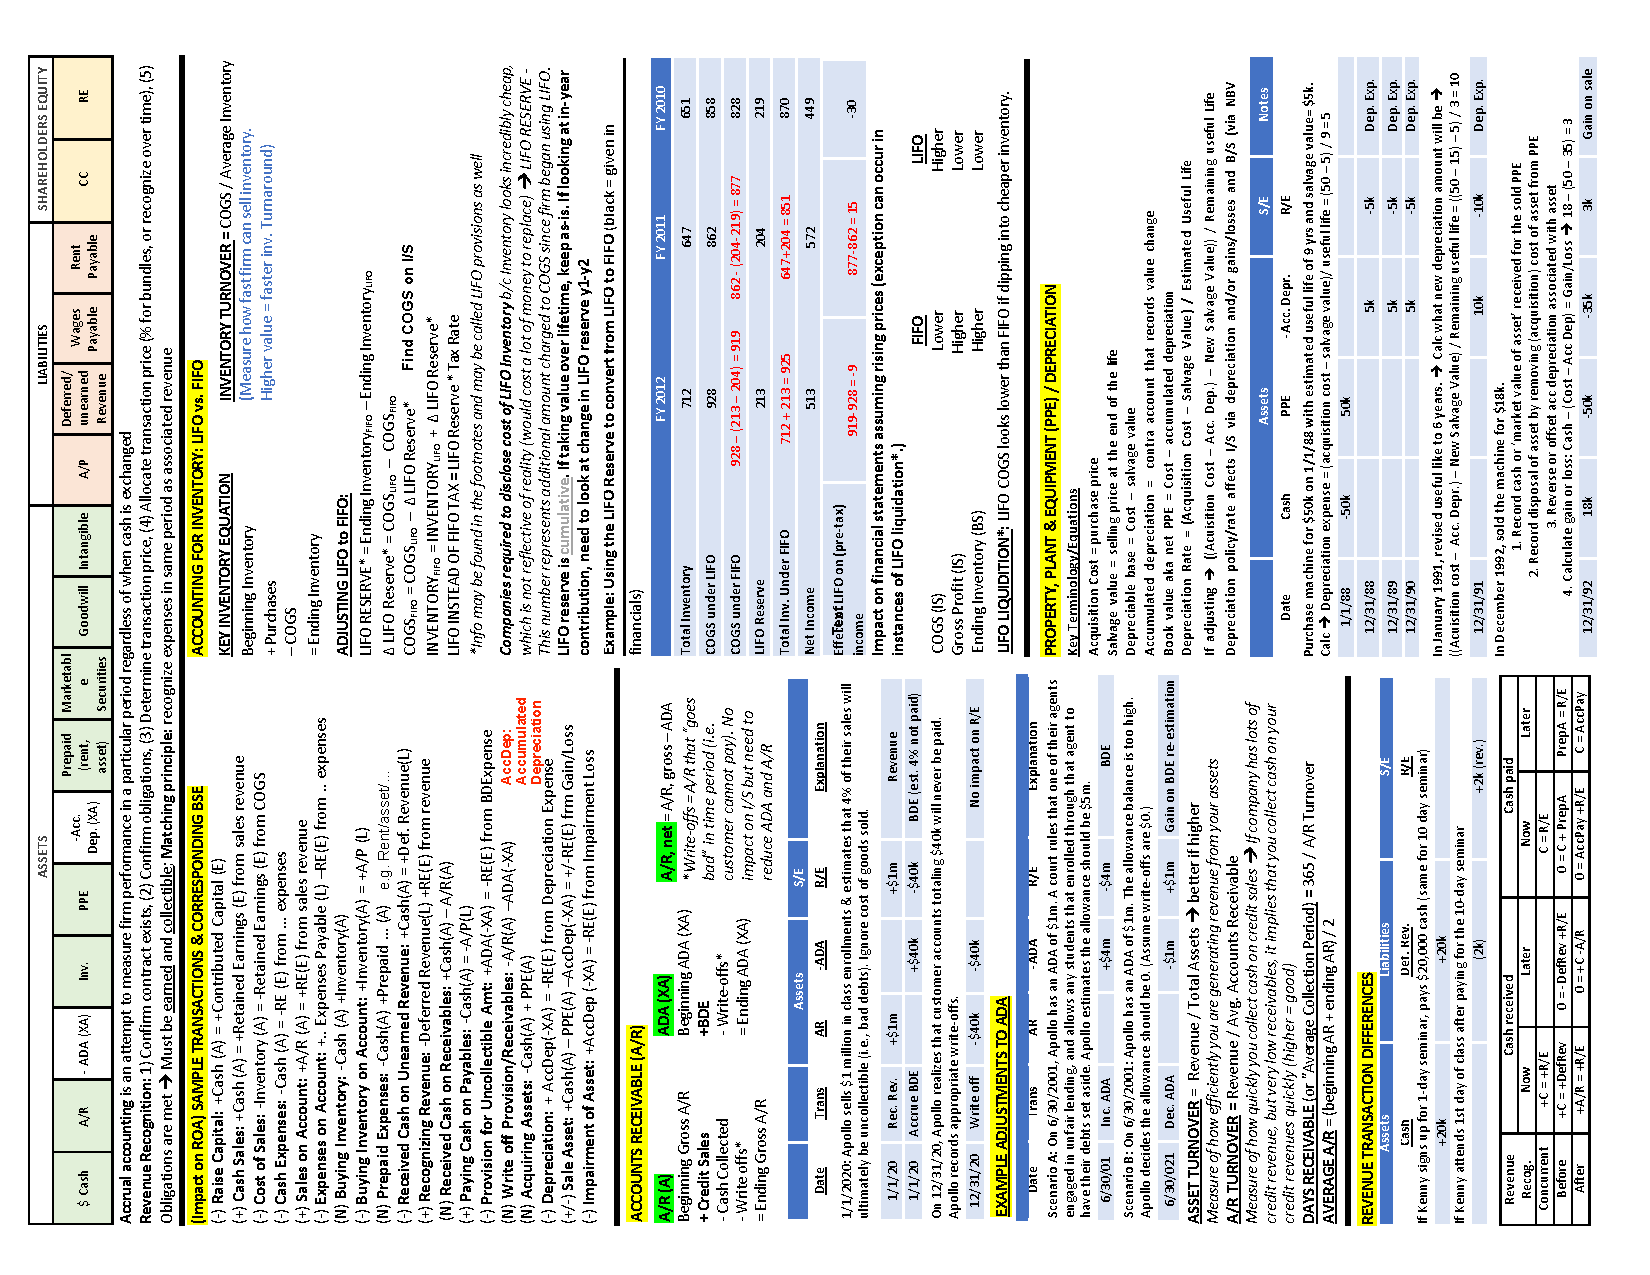
\includepdf[pages=-]{15_515_H1_Cheatsheet.pdf}

\end{document}